\documentclass [a4 paper,11pt]{report}
\usepackage [french]{babel}
\usepackage [utf8]{inputenc}
\usepackage{graphicx}
\usepackage[T1]{fontenc}
\usepackage{textcomp}
\usepackage{listingsutf8}
\usepackage{xcolor}
\usepackage{textcomp}
\usepackage{float}
\usepackage{hyperref}
\usepackage{fancyhdr}

\lstset{
inputencoding=utf8/latin1,
belowcaptionskip=1\baselineskip,
inputencoding=utf8/latin1,
breaklines=true,
frame=L,
xleftmargin=\parindent,
language=c++,
showstringspaces=false,
basicstyle=\footnotesize\ttfamily,
keywordstyle=\bfseries\color{purple!40!black},
commentstyle=\itshape\color{green!40!black},
identifierstyle=\color{black},
stringstyle=\color{blue},
}

\title {Compte rendu TP traiment d'images}
\author {
\bsc{LE PHILIPPE} Noé\\
}
\date{\today}

\begin{document}
\makeatletter
 
\maketitle
\section*{Algorithmes}

\subsection*{Lecture du fichier}
\begin{lstlisting}
void RawReader::load(std::string path) {
  std::ifstream f (path.c_str(), ios::in | ios::binary);
  unsigned short c;
  //chaque image est representee sous la forme
  //d'un tableau a une dimension de la taille de l'image
  unsigned short *img = new unsigned short [sizeX*sizeY];
  int i = 0;
  while(!f.eof()) {
    f.read((char *)&c,sizeof(short));

    //inversion des bits
    short l = c % 256;
    short r = c / 256;

    img[i++] = l * 256 + r;
    //lorsque la totalitee de l'image est lue
    //elle est ajoutee au vector d'images
    if(i >= sizeX * sizeY) {
      i = 0;
      data.push_back(img);
      img = new unsigned short [sizeX*sizeY];
    }
  }
}
\end{lstlisting}

\subsection*{Accès à une valeur}
\begin{lstlisting}
/**
Les images sont stockee dans un std::vector
Pour avoir le pixel à la couche k du fichier
on lit l'index k du std::vector
*/
unsigned short RawReader::getValue(int i, int j, int k) {
  return data[k][i * sizeY + j];
}
\end{lstlisting}
\newpage
\subsection*{Valeur maximum de l'image}
\begin{lstlisting}
/**
Parcours de tous les pixels de toutes les images
*/
unsigned short RawReader::getMaxValue() {
  unsigned short maxi = 0;
  for (int i = 0; i < sizeX; ++i) {
    for (int j = 0; j < sizeY; ++j) {
      for (int k = 0; k < sizeZ; ++k) {
        maxi = max(getValue(i, j, k), maxi);
      }
    }
  }
  return maxi;
}
\end{lstlisting}
\newpage
\section*{Volume Rendering}
Il n'y aura que les résultat du volume rendering sur WHATISIT, il serait redondant d'insérerer les résultats pour tous les fichiers alors que les algorithmes sont les mêmes.

\begin{figure}[h!]
\noindent\makebox[\textwidth]{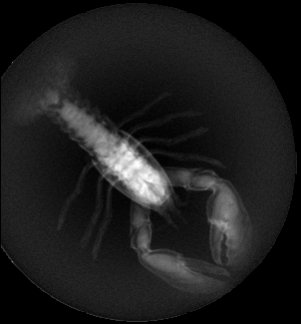
\includegraphics[width=200pt]{output/lobster_aip.png}}
\caption{Volume rendering : AIP}
\end{figure}

\begin{figure}[h!]
\noindent\makebox[\textwidth]{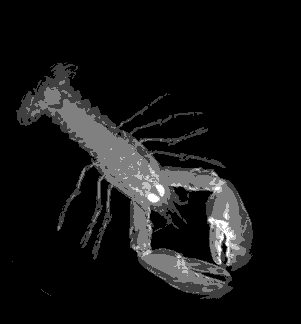
\includegraphics[width=200pt]{output/lobster_mip.png}}
\caption{Volume rendering : MIP}
\end{figure}

\begin{figure}[h!]
\noindent\makebox[\textwidth]{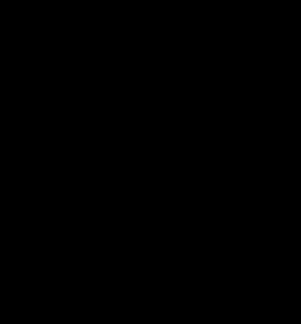
\includegraphics[width=200pt]{output/lobster_minip.png}}
\caption{Volume rendering : MINIP}
\end{figure}

\newpage
\section*{Code source}

\lstinputlisting[language=C++]{./RawReader.h}


\end{document}

